\documentclass{article}

\usepackage{graphicx}% Include figure files
\usepackage{color}
\definecolor{dkgreen}{rgb}{0,0.6,0}
\definecolor{gray}{rgb}{0.5,0.5,0.5}
\definecolor{mauve}{rgb}{0.58,0,0.82}
\usepackage{listings}
\lstset{frame=tb,
  language=Java,
  aboveskip=3mm,
  belowskip=3mm,
  showstringspaces=false,
  columns=flexible,
  basicstyle={\small\ttfamily},
  numbers=none,
  numberstyle=\tiny\color{gray},
  keywordstyle=\color{blue},
  commentstyle=\color{dkgreen},
  stringstyle=\color{mauve},
  breaklines=true,
  breakatwhitespace=true,
  tabsize=3
}




\begin{document}
\title{NLab Manual}
\author{Orkesh Nurbolat}
\maketitle

NLab is a python program used as an experiment managing program.
Designed to reduce human effort and be flexible for experiments. 
It is majorly writed in Python .

\section{General Idea}

\subsection{Problem when doing experiments}
~

Most of the experiments conducted at lab are 
	mainly scaning particular variables.
However when there are too many things to operate,
	it will be inconvinient to do it without a managing tool.
Take Labber for example. It is an exellent tool to do experiemnts.
However Labber follows convetional software designing principles,
	and it is comercial software.
The Labber system runs very bloated and it is un-operatable un-modifiable.
It heavily relay on GUI and tidious to operate. 
So the managing tool Labber is only suitable to run few small scale experiments
that is conventional and easy.

And for those who decide to directly use python to run experiments.
It might be the better choice for freedom and modifiability compared
to Labber.
However once the system gets complicated. It will also be tideous for
	the user to manage it. 
For example in the main loop of an experiemnt.
	If some variables are scanned as shown as



\begin{lstlisting}
A = np.linspace(0,10 ,200);
B = np.linspace(-5,5 ,200);
C = np.linspace(20,100 ,200);
for  a in A : 
	D = 5*a;
	for b in B: 
		E = D + b + 5 ;
		for c in C: 
			F = D * c ;
			//here do experiemnt
\end{lstlisting}

If I have to change some order for example put A bellow C.
Then there I have to do lots of efforts to have this completed.
Juts like shown here : 

\begin{lstlisting}
A = np.linspace(0,10 ,200);
B = np.linspace(-5,5 ,200);
C = np.linspace(20,100 ,200);
for b in B: 
	for c in C: 
		for  a in A : 
			D = 5*a;
			E = D + b + 5 ;
			F = D * c ;
			//here do experiemnt
\end{lstlisting}
So that when running in this kind of modes the user have to
manage the reliance of variables in thier code lines.
And handle the conflict between {\bf data flow order} and the {\bf execution order}.
Which makes doing experiment messy.

\subsection{Solution}
As mentioned above since  {\bf data flow order} and the {\bf execution order} 
	can conflict each other in python coding. 
We tried to design a system that only has {\bf data flow order} and the 
	{\bf execution order} is completely depreciated.
Since all the experiements condcuted in laboratory are semantically linked and
	indeed can be expressed as directed acyclic graph(DAG) of variable flow from
	settings to the instruemnts.
If one of the variable changes it only have to update all thouse decendent of this node. So that {\bf data flow order} abstraction is good enough to run almost every single experiment. We validated this in Lab and results are promissing.

By {\bf data flow order} we mean only managing the content of the data element, 
	as well as handling its relationship with other data elements. 
With this the system will figure out an execution order that is optimal. 
So that in the context of the user, 
	{\bf you only have to take care of values, you can write them in any order!}
So that your effort of doing experiments are dramatically decreased.

To execute such a system, a python dictionary like class is used to register all the values that have to be setted in an experiment. 
Lets call this dictionary ``g". so if the data flow theory is right. The example
wroten above could take the form as:

\begin{lstlisting}
g["D"] = " 5 * $A" 
g["E"] = " $D + $B + 5" 
g["F"] = " D * $C" 
g["A"] = vlin(0,10 ,200);
g["B"] = vlin(-5,5 ,200);
g["C"] = vlin(20,100 ,200);
g.run();
\end{lstlisting}

where this ``g" is the dictionary to register all the orderless values.
and ``vlin" is  special class that is latter recognized to linread scan the variable.
the dollar sign \$ means refering to a variable.
For example \$A means refering to the scanned variable A.
So later on just before ``g.run()" the variables registerd in ``g"
	is analysed and a runing order is decided.

Now if I have to change the order of A and C I just have to change it when the 
	vlin is assigned to them. Just like this : 

\begin{lstlisting}
g["D"] = " 5 * $A" 
g["E"] = " $D + $B + 5" 
g["F"] = " D * $C" 
g["C"] = vlin(20,100 ,200);
g["B"] = vlin(-5,5 ,200);
g["A"] = vlin(0,10 ,200);
g.run();
\end{lstlisting}
And the rest of the order are handeled just before the experiment running.

Since for the keys in values ``g" we only have to set values. 
We do not need to write any code to do this.
Despite the parts that have to scan the variables.
We can hold the rest in a dictionary like 

\begin{lstlisting}
{
	"D": " 5 * $A" ,
	"E": " $D + $B + 5" ,
	"F": " D * $C" 
}
\end{lstlisting}

{\bf So that these parts does not have to be writen into python code, 
	and they could be read out from json files.}
In fact when we are managing a large system, 
	most of the variables are writen in json and read from file just at the beging.
Only very important steps to setup is writed in code, 
	for example the scannings setted with ``vlin" above.
Or some settings to override the previous settings etc.
So that our main loop tend to be very short and clean.

{\bf And just because of this, we seperated massive 
	parameters and few lines of actuall experiment codes for the users.
	While managed them together so that we can conduct experiements
}
And we can manage thier relationships the way we wanted. 
	It is highly costumizable, effortless to use and flexible for all kinds of needs.
It is not a tool just for doing experiments in Lab, 
	infact if could be used in any contex that requires onlt data flow logics.
And mostly physical settups that has strong semantic relationship are very suitable
	for this Idea.


\section{Quick Start}
You should run 2 program.
One as your server. the other as your experiment platform Root (client)
	where you do whatever you want. 
A very important requirement is that these server and the platform Root(client)
	have to be consistent to each other.
That is why when they are created. They should load the same settings.
So that they can have good and great values.

The server is runned in a bare bone python cmd line or an ipython if perfered. 
And the Root part usually run in 
	``Jupyter Notebook",``Jupyter Lab" or ``vscode python". 
Do not run the server in these things since the server have to 
	spawn a few process which does not run properly in ``vscode python"

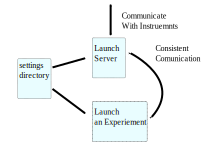
\includegraphics[width=\textwidth]{imgs/consistent.pdf}

\section{Settings}
	The settings is a folder which can recursivly be more folder inside another.
But at the end there will be readable json files.
{\bf There is no any restriction to write these settings}, 
	one should flow suggested good habits,
{\bf but this habit is not a requirement, so that we keep our 
	experiment volatile and has freedom to change}.

If S is ourserver, to tell it to load this settings directory, I just have
to tell it 
\begin{lstlisting}
S.load_dir("settings")
\end{lstlisting}
	in the server part , assuming ``S" is an server instance. 
And for the client part I also just have to write 
\begin{lstlisting}
g.load_dir("settings")
\end{lstlisting}
	assuming ``g" is a client instance (we call it Root).

In the end of these tree is the json file. just like we said
you can write anything inside this json file.
However, to be able to get these files recognized by Server ``S" and 
	Root ``g", you have to write some of these keys.

\begin{lstlisting}
NAME 
// a name that is assigned for this json file , as well used as the
// class instance name if this json file will produce a driver wrapper.
MODULE 
// if this is an instrument where to load it's driver's wrappers
// the MODULE is just a importable python file
CLASS 
// in that model file, which class exatly is required to be the driver

CREATE_INIT
// is expected to take a list of arguments
// when this json creates a instruemnt

ACTUAL_INIT
// is expected to take a list of actions 
// after this json creates a instruemnt
// so that the instrument is properly usable

CONNECT 
// wheather to connect this driver at server, if it is not connected
// all rest of the settings will not be readed by the Root

PHONEY 
// wheather pretend to connect this driver so that the Root still read rest
// of the settings but the driver setting value commands does not take effect

STAGING
// *********THE MOST IMPORTANT KEY************
// under this key everything will be readed to the client(ROOT) 
// as actions to do every single things

STAGING_IMEDIATE
// immediatly doing things and load the keys to the STAGING 
// for example read the csv and read all the key values to STAGING
// this is done at the loading time. not when everything is running.

MACRO
// some macros seted to alternate choices in the settings

ORDER
// for keys under the STAGING, forcefully deciding some orders that will be kept

MAP
// map some short key to long keys so that they can be used conviniently

IMPORT
// import things to the Root's context, but WILL reload 

IMPORT_ONCE
// import things to the Root's context, but WILL NOT reload 

RUN
// record what to record, what to save and misc things

\end{lstlisting}

\subsubsection{NAME, MODULE, CLASS, CREATE\_INIT, ACTUAL\_INIT}
These 5 keys are required to create a class. 
For example 
	there exists a json file somewhere under a foldere called "settings". 
And this is the whole content written inside it.
\begin{lstlisting}
{
	"CONNECT":true,
	"PHONY":true, 	
	"MODULE":"Instruments.CTek.EZQ",
	"CLASS":"CTEK_EZQ_BOX", 
	"NAME":"box1" ,
	"CREATE_INIT":[],
	"ACTUAL_INIT":{
		"connect_Master":["Master" , "10.0.200.110"], 
		"connect_XY":[
			["AB" , "10.0.200.111"], 
			["CD" , "10.0.200.112"]
		],
		"connect_Z":[
			["Z1" , "10.0.200.113"]
		],
		"connect_ADC":[
			["ADC1", "A4-BB-6D-AA-2D-28","00-00-00-00-00-53" ]
		]
	}  
}
\end{lstlisting}
These contents are loaded to server when we are running the command in server
side :


\begin{lstlisting}
from NLab import * ;
S = Server(3232); // giving the server a port,same as client side
S.load_dir("settings");
S.main();
\end{lstlisting}

The settings here suppose to load a CTek box to the server.
The wrapper(driver) it is using is a importable file at "Instruments.CTek.EZQ".
And the exact class to creat this wrapper(driver) in that importable file is 
"CTEK\_EZQ\_BOX".
And the instance we are going to create is called "box1".
And when we create this "box1" we do not need to pass anything to it, 
	as there at "CREATE\_INIT" there appears nothing.
Later on we do lots of sub instrument loading at the key "ACTUAL\_INIT".
Real functional parts are loaded here.

The keys that appears like 
\begin{lstlisting}
"connect_Master":["Master" , "10.0.200.110"], 
\end{lstlisting}
where "connect\_Master" is a function defined previously in this wrapper.
and ["Master" , "10.0.200.110"]  are two arguments passed to this function.
In another word for the server, the things set above are equivalent to python code

\begin{lstlisting}
from importlib import reload ;
CONNECT = True ;
PHONEY = True;
if(CONNECT and not PHONEY):
	import Instruments.CTek.EZQ;
	reload(Instruments.CTek.EZQ);
	box1 = 	Instruments.CTek.EZQ.CTEK_EZQ_BOX();
	box1.connect_Master("Master" , "10.0.200.110") ;  
	box1.connect_XY(
			["AB" , "10.0.200.111"], 
			["CD" , "10.0.200.112"]
	);
	box1.connect_Z(
			["Z1" , "10.0.200.113"]
	);
	box1.connect_ADC(
			["ADC1", "A4-BB-6D-AA-2D-28","00-00-00-00-00-53" ]
	) 
\end{lstlisting}
Now , say this json file is stored at "settings/instr/b1.json", to address this instrument from the Root(cleint), I will write the key:

\begin{lstlisting}
g["!instr-box1"]
\end{lstlisting}
Note that there is a climax ahead of the key. Marking that this key will be sent
to the server, it is required for all the keys that have to be sent.
the "instr" is father folder for the json file "b1.json", {\bf THAT IS WHY
THIS "instr" followed by a dash line "-" is added before "box1"}.
the json file name "b1.json" is not important and could be anything.
However this instance has a name and it is called "box1", so that is why
we write here "!instr-box1".


Now what if I put my json file at another random place "settings/instr/boxes/left/b1.json".
Then I have to addres this instrument via key and command
\begin{lstlisting}
g["!instr-boxes-left-box1"]
\end{lstlisting}

Now if I have to address this "AB" instrument, 
I will write 
\begin{lstlisting}
g["!instr-boxes-left-box1-AB"]
\end{lstlisting}
we know this "AB" thing is acutally an 4 channel awg. with each 2 of them
connected to a IQ mixer.
and there are function "wave0" and "wave1" predefiend to set these 2 complex channels waves. And to actually do that( not do imediatly, but to register this and when "g.run()" is called it will do it), we suppose to write :

\begin{lstlisting}
from NLab import * ;
g=Root("localhost:3232"); g.load_dir("settings");
g["complex_wave1"] = np.sin(np.linspace(0,10,20000))
		+ 1j*np.cos(np.linspace(0,10,20000));
g["complex_wave2"] = """
	np.sin(np.linspace(0,10,20000))
	+ 1j*np.cos(np.linspace(0,10,20000))
""";
g["!instr-boxes-left-box1-AB-wave0"] = "$complex_wave1"
g["!instr-boxes-left-box1-AB-wave1"] = "$complex_wave2"
g.run();
\end{lstlisting}
Where this "complex\_wave1" and "complex\_wave2" are complex wave.
And they are sent to from the Root(client) "g" to the server "S".
and from "S" to the actual box and its AWG. And congratualtions!
you have learned exactly how to send a wave with NLab. And
do please try this out to see if this works.

One thing to notice is that the commad 

\begin{lstlisting}
g["complex_wave1"] = np.sin(np.linspace(0,10,20000))
		+ 1j*np.cos(np.linspace(0,10,20000));
\end{lstlisting}
	will compute the result immediatly and put it in the "g".
But the command
\begin{lstlisting}
g["complex_wave2"] = """
	np.sin(np.linspace(0,10,20000))
	+ 1j*np.cos(np.linspace(0,10,20000))
""";
\end{lstlisting}
	this key is assigned with actaully a string.
Since all the strings will be evaluated at the run time in this "g".
Here it will as well, so it is computed at run time instead of done
	immediatly.

To actaully write a string in g, this way does not work and will give error

\begin{lstlisting}
g["this_should_be_string"] = "the string"
\end{lstlisting}
The correct way to write it is like this 
\begin{lstlisting}
g["this_should_be_string"] = "'the string'"
\end{lstlisting}
Since, like said previously, every string will be evaluated in "g".
Another thing to notice is that the key 
\begin{lstlisting}
g["complex_wave2"] 
\end{lstlisting}
did not add any climax infront of it. Because there is
no consistent server that accepts it and it does not have to send this key to the server.


\section{STAGING}
if you saw above when we write the key 
\begin{lstlisting}
g["!instr-boxes-left-box1-AB-wave0"] = "$complex_wave1"
g["!instr-boxes-left-box1-AB-wave1"] = "$complex_wave2"
\end{lstlisting}
that key "instr-boxes-left-box1-AB-wave1" is pretty long.
And we need to write these things in settings files. instead not the code! 

Now how do we actually add this thing to the Setting json? 
The answer is really simple. please take a look at this example

\begin{lstlisting}
{
	"CONNECT":true,
	"PHONY":true, 	
	"MODULE":"Instruments.CTek.EZQ",
	"CLASS":"CTEK_EZQ_BOX", 
	"NAME":"box1" ,
	"CREATE_INIT":[],
	"ACTUAL_INIT":{
		"connect_Master":["Master" , "10.0.200.110"], 
		"connect_XY":[
			["AB" , "10.0.200.111"], 
			["CD" , "10.0.200.112"]
		],
		"connect_Z":[
			["Z1" , "10.0.200.113"]
		],
		"connect_ADC":[
			["ADC1", "A4-BB-6D-AA-2D-28","00-00-00-00-00-53" ]
		]
	}  
	"STAGING":{
		"!trig_interval":"100u"			,
		"!trig_count": "2k",
		"!depth"	:2000,
		"!Read-setup":["$depth", [ "120M" , "92.3M", 130e6, 112e6, 110e6, 90e6, 40e6]],
		"!Master-setArm":[true,false],
		"!AB-setArm":[false,false],
		"!CD-setArm":[false,true],
		"!Z1/setArm":[false,false,false,false] ,
		"!Master-trigDel": "50.1u" ,
		"!Master-outDel": "50u", 
		"!AB-trigDel": "0u",
		"!AB-outDel" : "0u", 
		"!CD-trigDel": "0u",
		"!CD-outDel" : "0u" ,
		
		"!AB-wave0":"np.array(np.linspace(0,50u,24k))",
		"!AB-wave1":"np.array(np.linspace(0,50u,24k))",
	}
}
\end{lstlisting}

As we are planned this json can appear any
place where it was planted it in settings directory.
Its purpose is to tell the server to open such an instrument.
And then pass every key-value pair under the STAGING directly
	to the Root. 
So  obiviously we notice the key {\bf "!AB-wave1"} at the 
	end of the STAGING session. 
And depending on where the json was in the setting. Its value {\bf"np.array(np.linspace(0,50u,24k))"}, is writen to key

\begin{lstlisting}
g["!instr-boxes-left-box1-AB-wave1"]
\end{lstlisting}

In another word.
Writing
\begin{lstlisting}
"!AB-wave0":"np.array(np.linspace(0,50u,24k))",
"!AB-wave1":"np.array(np.linspace(0,50u,24k))",
\end{lstlisting}
In the STAGING section of a file.
Is equivalent to write 
\begin{lstlisting}
g["!instr-boxes-left-box1-AB-wave0"] ="np.array(np.linspace(0,50u,24k))",
g["!instr-boxes-left-box1-AB-wave1"] ="np.array(np.linspace(0,50u,24k))",
\end{lstlisting}
And that is exactly the purpose of the STAGING section : to write lines and lines of python code back into the json.

Some one will ask why even bother to do things this way.
The json does not even have that high-lighting 
	or REPL utilities for Python.
Well that is true. 
However Python is a {\bf instruction flow }  program.
Which means it can not handle it's {\bf instruction flow } 
	and {\bf data flow } conflicts by itself.

However when we write these python lines in to the STAGING sections.
{\bf Their order are relative } so that it can handle 
	all the confilcts by itself. Unless there are looped definitions.

Now for the other keys in the STAGING section they are basically same.
So suddenly If I like to change my trigger count in code instead of
	in the json file. 
All I have to do is this.
\begin{lstlisting}
g["!instr-boxes-left-box1-trig_count"] = "5k"
\end{lstlisting}

This key "!instr-boxes-left-box1-trig\_count"  is really long, And please
take a look at the "MAP" section that is designated for json to shorten
this key length. And what does that "5k" means, please take a look at the Abbrivation section

\section{Abbreviation of orders}
To be able to comfortly do experiments we like to 
	abbreviate some number orders.
Since in our system if you write string in the json key,
	it will be evaluated.
Taking this as an advantage we could write things like this in the key:


\begin{lstlisting}
"!AB-wave0":"np.array(np.linspace(0,50u,24k))",
"freqs":["654.543M","-45M","44M**2"],
"amps":["121m","43m","220m"]
\end{lstlisting}

And they are equivallent with :

\begin{lstlisting}
"!AB-wave0":"np.array(np.linspace(0,50/1000_000,24*1000))",
"freqs":["654.543*1000_000","-45*1000_000","(44*1000_000)**2"],
"amps":["121/1000","43/1000","220/1000"]
\end{lstlisting}


And in the here all those number order abbriviations
are listed.
\begin{lstlisting}
  'f': '/ 1000_000_000_000_000 ',
  'p': '/ 1000_000_000_000 ',
  'n': '/ 1000_000_000 ',
  'u': '/ 1000_000 ',
  'm': '/ 1000 ',
  'k': '* 1000 ', 
  'K': '* 1000 ',
  'M': '* 1000_000 ',
  'G': '* 1000_000_000 ',
  'T': '* 1000_000_000_000 ' , 
  'P': '* 1000_000_000_000_000'
\end{lstlisting}


\section{Mapping}
Some keys in the STAGING parts of the json file is 
	little bit too long.
For example  this key

\begin{lstlisting}
g["!instr-boxes-left-box1-trig_count"] = "2k"
\end{lstlisting}
And in a NLab json, there is special section called MAP,
where we can map longer keys to shorter keys.


\begin{lstlisting}
{
	"MAP"	:{
		"tc":"instr-boxes-left-box1-trig_count"
	}
	...	
	"MODULE":"Instruments.CTek.EZQ",
	"CLASS":"CTEK_EZQ_BOX", 
	...	
	"STAGING":{
		...	
		"!trig_interval":"100u"			,
		...	
	}
}
\end{lstlisting}
Where this ... is trival repeat of parts in previous examples.
And one very quickly notices that the map is corresponding with
	one of the STAGING key. 
However when doing mappings the key is writen in full path .
Now back in the code part that manipulates the Root. 
If I have to  change trigger count, All I need to do is:

\begin{lstlisting}
#/*g["!instr-boxes-left-box1-trig_count"] = "5k"*/
g["!tc"] = "5k"
\end{lstlisting}
and because the key "tc" is mapped, 
	it is equivalent with the part that is commented.

\subsection{Using one instrument's key in another instrument}
If a key is mapped, it is writen in full path .
And this kind of mapped keys can be called in STAGING that bellong to
other json files, without mistaken as thier keys.
For example if I summon the AWG instrument in the settings/instr/box.json .
Now I had to set this exact AWG insturment's key at settings/qubits/waves.json 
This is what I will do : 

\begin{lstlisting}
// settings/def/map.json
// this json file is purposed to enumerate 
// all the mappings so that I could manage them easily 
// mapping could be writen in multiple files as well
// it does not matter because every map is full path
{ 
	"MAP"	:{
		...	
		"tc":"instr-boxes-box1-trig_count"
		"AB0":"instr-boxes-box1-AB-wave0"
		"AB1":"instr-boxes-box1-AB-wave1"
		...	
	}
}
\end{lstlisting}



\begin{lstlisting}
// settings/instr/box.json
// same as the previous examples but the mappings are not
// writen seperatly and all collected to settings/def/map.json
// instead
{ 
	...	
	"MODULE":"Instruments.CTek.EZQ",
	"CLASS":"CTEK_EZQ_BOX", 
	...	
}
\end{lstlisting}



\begin{lstlisting}
// settings/qubit/wave.json
// same as the previous examples but the mappings are not
// writen seperatly and all collected to settings/def/map.json
// instead
{ 
	"STAGING"{
		...	
		"!AB0":"$wave0",
		"!AB1":"$wave1"
	}
}
\end{lstlisting}

So that the key "!AB0" that actually bellong to the staging
part of the settings/instr/box.json now is used in the 
settings/qubit/wave.json 's STAGING section


\subsection{mapping with hierarchy}
Mapping can be done at your own will.
Based on our experiment experience. We happened to map 
the keys centerd to qubits.
We say this qubits this and this qubits that.
And this kind of mapping could be expressed as bellow

\begin{lstlisting}
{
	"MAP":{
		"q0":{
			"awg":"instr-box1-AB-wave0",
			"lo":{ // drive local
				"freq":"instr-drlo1-freq",
				"power":"instr-drlo1-power",
			}
			"pr":{ // probe local
				"freq":"instr-prlo1-freq",
				"power":"instr-prlo1-power",
			}
			"trace":"trace-put~q0" // display
		}
		
		"q1":{
			"awg":"instr-box1-AB-wave1",
			"lo":{ // drive local
				"freq":"instr-drlo1-freq",
				"power":"instr-drlo1-power",
			}
			"pr":{ // probe local
				"freq":"instr-prlo1-freq",
				"power":"instr-prlo1-power",
			}
			"trace":"trace-put~q1" // display
		}
	}
}
\end{lstlisting}

Now to assign value to them, I could write in {\bf any} json file's STAGING section 


\begin{lstlisting}
{
	...
	"STAGING":{
		...
		"!q0-awg":"$wave0",
		"!q0-trace":["$wave0"...],
		"!q1-awg":"$wave1",
		"!q1-trace":["$wave1"...],
		"!q1-lo-power":20,
		"!q1-lo-freq":"6.95G",
		...
	}
	...
}
\end{lstlisting}
{ \bf Note that the mapped key will not hierachialy make up to be full path again ,since it already has been writen in full path when mapped.}


\section{Order}
Under the section ORDER your could write
 keys that suppose to be conducted conseqeuntly.
 For example the CTEK awg have to resend waveform if it changed the 
 offset.
This is not handled by the driver.
So I can just force to let this order exist.





\begin{lstlisting}

{
		...
    "STAGING":{
				...
        "!Master-offset":["$ProA/offset_I","$ProA/offset_Q","$ProB/offset_I","$ProB/offset_Q"],
        "!AB-offset":["$XYA1/offset_I","$XYA1/offset_Q","$XYB1/offset_I","$XYB1/offset_Q"],
        "!CD-offset":["$XYC1/offset_I","$XYC1/offset_Q","$XYD1/offset_I","$XYD1/offset_Q"],
        "!EF-offset":["$XYA2/offset_I","$XYA2/offset_Q","$XYB2/offset_I","$XYB2/offset_Q"],
        "!GH-offset":["$XYC2/offset_I","$XYC2/offset_Q","$XYD2/offset_I","$XYD2/offset_Q"],   
        "!Z1-offset":[1040,-200, 230, 210],
        "!Z2-offset":[490, 350, 470, 400] ,

        "!Z1-wave0":"np.zeros(128)" ,
        "!Z1-wave1":"np.zeros(128)" ,
        "!Z1-wave2":"np.zeros(128)" ,
        "!Z1-wave3":"np.zeros(128)" ,
        "!Z2-wave0":"np.zeros(128)" ,
        "!Z2-wave1":"np.zeros(128)" ,
        "!Z2-wave2":"np.zeros(128)" ,
        "!Z2-wave3":"np.zeros(128)" ,
        "!AB-wave0":"np.zeros(128,dtype=complex)" ,
        "!AB-wave1":"np.zeros(128,dtype=complex)" ,
        "!CD-wave0":"np.zeros(128,dtype=complex)" ,
        "!CD-wave1":"np.zeros(128,dtype=complex)" ,
        "!EF-wave0":"np.zeros(128,dtype=complex)" ,
        "!EF-wave1":"np.zeros(128,dtype=complex)" ,
        "!GH-wave0":"np.zeros(128,dtype=complex)" ,
        "!GH-wave1":"np.zeros(128,dtype=complex)" 
    } , 
    "ORDER":[
        ["!Master-offset" ,"!Master-wave0"  ] , 
        ["!Master-offset" ,"!Master-wave1" ] ,
        ["!AB-offset" ,"!AB-wave0"  ]  , 
        ["!AB-offset" ,"!AB-wave1" ] ,
        ["!CD-offset" ,"!CD-wave0" ] , 
        ["!CD-offset" ,"!CD-wave1" ] ,
        ["!EF-offset" ,"!EF-wave0" ] , 
        ["!EF-offset" ,"!EF-wave1" ] ,
        ["!GH-offset" ,"!GH-wave0" ] , 
        ["!GH-offset" ,"!GH-wave1" ] ,
        ["!Z1-offset" ,"!Z1-wave0" ] , 
        ["!Z1-offset" ,"!Z1-wave1" ] ,
        ["!Z1-offset" ,"!Z1-wave2" ] , 
        ["!Z1-offset" ,"!Z1-wave3" ] ,
        ["!Z2-offset" ,"!Z2-wave0" ] , 
        ["!Z2-offset" ,"!Z2-wave1" ] ,
        ["!Z2-offset" ,"!Z2-wave2" ] , 
        ["!Z2-offset" ,"!Z2-wave3" ] ,  
        ["!ADC1-start" , "!ADC1-freqs"],
        ["!ADC1-width" , "!ADC1-freqs"]
    ]
}

\end{lstlisting}
Just becuase the ORDER section, now if my offset is changed
it will automatically resend the wave.





\section{Keys that must be called more than once}


Since we organize things to be done in a dictionary.
In a dictionary, for one key there could only have one value entry.

However sometimes we have to call keys mulitple times with 
	different values to complete setup.
For example

\begin{lstlisting}
{ 
	"STAGING"{
		"!tracer-put"	:["'wave0'",0,["$wave0[0]","$wave0[1]"]]
		"!tracer-put"	:["'wave1'",1,["$wave1[0]","$wave1[1]"]]
	}
}
\end{lstlisting}

The command above suppose to put two waveform 
	on to the tracer display.
However if I persisted with the way I wrote. Only the latter
	one will be displayed, since it covered that same key setted
	right before it.
I  like to see both of them, and this is what I should do:

\begin{lstlisting}
{ 
	"STAGING"{
		"!tracer-put~dsafs"	:["'wave0'",0,["$wave0[0]","$wave0[1]"]]
		"!tracer-put~543543"	:["'wave1'",1,["$wave1[0]","$wave1[1]"]]
	}
}
\end{lstlisting}

And now it is perfect, these both are going to be displayed.
What you should notices is that there is $\sim$ .
And the part after the $\sim$ in the keys above are different,
	so that these two key can be tell apart.
Latter, when this keys are suppose to be take effect, In another
	word actually sent to the instrument. the part that is affter the 
$\sim$ is cut down.
So that the key "tracer-put" is called twice correctly.

\section{Key Value Reference System}
Every key directly under the STAGING are eventually stored parallel 
	and later on this level they are sorted and executed.
So every key directly under the STAGING are the atom of operations.
If the value of a key is a nested structure of other parts.
The inside execution order will not be sorted and will remain.


\subsection{split mark for keys}
say there are some where in whatever json file, has its STAGING section looks like this : 
\begin{lstlisting}
{
	"NAME":"lop"
	"STAGING":{
		"A":{
			"B":432423
		}
	}
}
\end{lstlisting}
where "A" is a key that is directly under STAGING,
while "B" is indirectly under this staging, it is firstly under "A".
Now I like to use the value in "B" and assign it to "C".
\begin{lstlisting}
{
	"NAME":"lop"
	"STAGING":{
		"A":{
			"B":432423,
			"C":"$B"
		}
	}
}
\end{lstlisting}
since "B" is directly neighbor to "C", the reference could be wroten this way. And that is equivalent with writing
\begin{lstlisting}
{
	"NAME":"lop"
	"STAGING":{
		"A":{
			"B":432423,
			"C":"$A/B"
		}
	}
}
\end{lstlisting}

But, If I write this way : 
\begin{lstlisting}
{
	"NAME":"lop"
	"STAGING":{
		"A":{
			"B":432423,
			"C":"$lop-A['B']"
		}
	}
}

\end{lstlisting}

It is refering to "lop-A" correctly, and taking the "B"
key under the "lop-A". However it is a error in this example
because it is "lop-A" now is refering to it self. It is a loop
defintion. if there is no loop then it is acutally OK to do this.

To be able to avoid the loop issue, one can write this way.
\begin{lstlisting}
{
	"NAME":"lop"
	"STAGING":{
		"A":{
			"B":432423,
			"C":"$lop-A/B"
		}
	}
}
\end{lstlisting}
Where this "/" means next hierachy in the sub dictionary.
It should not be mixed with the "-" where "-" is
used to express hierachy from the root of setting until the direct key under STAGING section. And from the key in the STAGING to bellow strucuture , hierachy is expressed with "/". If there is no loop, you could have just used "[]" like the good old way in python. It works.


If that "C" key above actually did not exist.
And I wanted to create it in the Root code part.
I can just do it like this : 

\begin{lstlisting}
g["lop-A"]["C"] = "$lop-A/B";
\end{lstlisting}


Now If I write
\begin{lstlisting}
{
	"NAME":"lop"
	"STAGING":{
		"A":{
			"B":432423,
			"C":"$B"
		}
		"D":"$B"
	}
}
\end{lstlisting}
at the key "D" , it does not have a brother called "B", So this reference can not find the correct key, and thus it will be an error.
To write this "D" correctly I should write

\begin{lstlisting}
{
	"NAME":"lop"
	"STAGING":{
		"A":{
			"B":432423,
			"C":"$B"
		}
		"D":"$A-B"
	}
}
\end{lstlisting}
or
\begin{lstlisting}
{
	"NAME":"lop"
	"STAGING":{
		"A":{
			"B":432423,
			"C":"$B"
		}
		"D":"$lop-A['B']"
	}
}
\end{lstlisting}

\subsection{split mark}
So as shown in the  example above.
"/" is the hierachy for keys of things direct under "STAGING".
For list hierachy one could just wrote "/\#index" ,where this "index"
can be replaced with constant numbers, for example
\begin{lstlisting}
{
	"NAME":"lop"
	"STAGING":{
		"A":{
			"B":432423,
			"C":"$B"
			"K":[43e5,321e6,"20G"],
		}
		"D":"$lop-A/K/#2"
	}
}
\end{lstlisting}
So that this "D" is refering to the "20G" at the "A/K" key.
And of course you could have just wrote, since you do not
have to worry about refering to itself issue here.

\begin{lstlisting}
{
	"NAME":"lop"
	"STAGING":{
		"A":{
			"B":432423,
			"C":"$B"
			"K":[43e5,321e6,"20G"],
		}
		"D":"$lop-A['K'][2]"
	}
}
\end{lstlisting}

And if there is 


\begin{lstlisting}
{
	"NAME":"lop"
	"STAGING":{
		"A":{
			"B":432423,
			"C":"$B"
			"K":[43e5,321e6,"20G"],
		}
		"D":"$lop-A['K'][2]"
		"E":"$dop-nop-shop-xyz"
	}
}
\end{lstlisting}
where this "E" key is special.
and there "dop-nop-shop-xyz" is not find in this file's staging , so it is an {\bf external reference} ,and
it have to be writen at "settings/dop/nop/shop/ffdsfdsf.json"  with no NAME section in this "ffdsfdsf.json"  or writen in "settings/dop/nop/ffdsfdsf.json" with a name section and this name section is "shop" .

No matter what, that "xyz" is a direct key under that json file's STAGING section.

\subsection{making keys that are easy to grab}
A good habit when we say "grab" by the key. we mean create this key so that it is both efficeint and convinent so start scanning from this key.
for example, lets say for human readable sake, we put all the frequencies of qubits together like

\begin{lstlisting}
{
	"STAGING":{
		"freqs":[5641310844.361463,6249702327.724407,5543070607.445814,6271764823.07361,5610179403.893467,6264466031.663818,5621323460.449283,6148057807.784958],
		"piwidth":[3e-08,3e-08,3e-08,3e-08,3e-08,3e-08,3e-08,3e-08],
		"piamp":[0.14134881253739687,0.3472308068031981,0.21957048873722318,0.20445849268925745,0.1370432338043951,0.18301346995335352,0.17112939731078053,0.5],
		"drag_scale":[5.382962092344444e-12,-3.4447432003088383e-10,-5.954827722424791e-10,-1.324816513163791e-10,4.683439251885672e-10,-8.905277110136361e-11,1.1041760585846665e-09,0],
		"pi2ratio":[0.9961835407284517,0.9912226367586031,0.9917845620209382,0.9946672480931976,0.9956273996891115,1.0072530470055292,1.0041945485470531,1],
		"drag2scale":[4.005297872882497e-11,-3.233439175531994e-11,-8.767757265279771e-10,2.538778275920134e-11,6.250925009434997e-10,-9.930423375603122e-11,2.385898674089222e-09,0],
		"pi_phase_misalign":[0.014002592454735127,0.005448319702750673,-0.014325645896390824,0.017884424793861587,0.0018187844002523453,-0.041835706582785154,0.060822719261248825,0],
		"anhar":[-266.4e6,-253.75e6,0,-253.7e6],
		"12piamp_scale":[1.04,0.8,0,0.86],
		"drag_detun":[
			[0,0],
			[0,0],
			[0,0],
			[0,0],
			[0,0],
			[0,0],
			[0,0],
			[0,0]
		]
	}
}

\end{lstlisting}

It will be easy for me to grab and scan any of these frequencies like

\begin{lstlisting}
g["qubits-freqs"][0] = vspn("5.6G" , "10M",201)
\end{lstlisting}

\section{IMPORT and IMPORT\_ONCE }
if you have something that you want only import once and
{\bf DO NOT RELOAD} , you should write them in IMPORT\_ONCE section.
but If you have something that you want everytime Root "g" 
load the setting it will {\bf RELOAD} it. you should
write that in the IMPORT section. for example : 
\begin{lstlisting}
	"IMPORT_ONCE":{
			"numpy":"np", // import numpy as np
			"NLab.Utils.common": "cm", // import NLab.Utils.common as cm
			"NLab.PulseGen.rb":"rb" ,
			"NLab.PulseGen.rb2":"rb2"
	} ,
    "IMPORT":{
				"My_tools.basic_pulses" : "bp" ,
				"NLab.PulseGen.rule4": "", // from NLab.PulseGen.rule4 import * 
				"My_tools.num2binary" : "",
				"My_tools.mygates" : "",
				"My_tools.mypulses" : "",
				"toolfunc.state_discriminator_gmm" : "sd" ,
				"misc":"", // from misc import * 
				"My_tools.loadcsv":""
    } ,
\end{lstlisting}
where this key is the python module. and the value is the module's name after import, its meaning is written in the comment above.
the 


\section{RUN}
in the RUN section you have to provide information
about how do you going to run/save/display your experiment.
And these are the keys your have to set

\begin{lstlisting}
{
	"RUN":{
		"TRACE":{
			// The trace like data
			// it returns  a trace of results when one step of
			// experiment is conducted
		}
   
		"POINT":{
			// The point like data
			// it returns  a single point of results when one step of
			// experiment is conducted
		}

		"SAVE_PATH_MAJ": // the major save path
		"SAVE_PATH_MNR": // concated to SAVE_PATH_MAJ and become 
			// "SAVE_PATH" is the place where data is saved
		"DIR_TO_SAVE":// a list of directory to be saved when experiment started ,
		"FILE_TO_SAVE":// a list of file to be saved when experiment started,
		"ACTIONS" : // a list of trigger keys that required before acquizition ,
		"DELAY": // a delay in second ,
		"TOKEN_KEY": // a instrument key that is set when a fragment of experiemnt ends,
		"PLOTER":// instantaneous data displayer
	}
}

\end{lstlisting}


a typical example for this is like 
\begin{lstlisting}
{
	"RUN":{
		"TRACE":{
        "S0":"&instr-zi-qa1-S0"  ,
        "S1":"&instr-zi-qa1-S1"  ,
        "S2":"&instr-zi-qa1-S2"  ,
        "S3":"&instr-zi-qa1-S3"  ,
        "S4":"&instr-zi-qa1-S4"  ,
        "S5":"&instr-zi-qa1-S5"  ,
        "S6":"&instr-zi-qa1-S6"  ,
        "S7":"&instr-zi-qa1-S7"
		}
   
		"POINT":{
        "A0":"np.mean(&instr-zi-qa1-S0)"  ,
        "A1":"np.mean(&instr-zi-qa1-S1)"  ,
        "A2":"np.mean(&instr-zi-qa1-S2)"  ,
        "A3":"np.mean(&instr-zi-qa1-S3)"  ,
        "A4":"np.mean(&instr-zi-qa1-S4)"  ,
        "A5":"np.mean(&instr-zi-qa1-S5)"  ,
        "A6":"np.mean(&instr-zi-qa1-S6)"  ,
        "A7":"np.mean(&instr-zi-qa1-S7)"
		}

		"SAVE_PATH_MNR":"test\\test",
		"SAVE_PATH_MAJ":"DATA",
		"DIR_TO_SAVE":["settings"],
		"FILE_TO_SAVE":[ "Tqg2.ipynb","Floquet Ising.ipynb","PROC_TQG.ipynb" ] ,
		"ACTIONS" :["instr-zi-run" ] ,
		"DELAY":0.001,
		"TOKEN_KEY": "instr-dview-roll",
		"PLOTER":"instr-dview"
	}
}
\end{lstlisting}
where this "\&"  is alike to "\$" , but now it means 
this key is a readable key and read value from it.
here "instr-zi-qa1-S5" is a function of Zurich instrument driver
that suppose to return the single shot array of qubit 5.
The definition of this function is in the wrapper of Zurich instrument.
And the key "instr-zi-run" is the key what we will do before
doing aquizition.
And the key "instr-dview" is the name of the data displayer.





\section{RUNNING experiments}
\subsection{vlin,vspn}
this two class is used to linear start-stop and center-spand scan things.

It can be used as following : 

\begin{lstlisting}
g=NLab.Root("localhost:3232");g.load_dir("settings")
g["A"] = vlin(0,20,40);
g["B"] = vspn(0,4,40);
g.run("C",True)
\end{lstlisting}
This will scan the "A" and "B" accordingly and save the data
for the option of "g.run" please check the Root.run function bellow



\section{Optimizing}
\subsection{opt}
this class is used as tool to optimize entry for experiments.
it accept one parameter to tell which argument to 
take as an entry for this key variable.
for example
\begin{lstlisting}
g["A"] = opt(0);
g["B"] = opt(1));
g["C"] = "$C**2 + ($A+1)**2";
\end{lstlisting}
makes "A" the first entry for the funcion , and "B" the second one.
There is no limit how much of them can be used.
However when they are used. No any "vlin" or "vspn" 
can be used with them .

\subsection{minimizing}
for example
\begin{lstlisting}
g=NLab.Root("localhost:3232");g.load_dir("settings")
g["A"] = opt(0);
g["B"] = opt(1));
g["C"] = "$C**2 + ($A+1)**2";
g.setup_opt(lambda r : np.mean(r.DATA["C"])  );
scipy.optimize.minmize(g.opt_function2 , [2,3]);
\end{lstlisting}

where this "g.setup\_opt" function will setup this root to be optimized.
it requires a function that must return a scalar so that it could be optimized by scipy optimizer.
So that every time "g.opt\_function2" can be called
and it will require 2 arguments







\section{Root Asset and Function Specification}
usually we call it "g" in the coding

\subsection{Root.run(option, block=False)}
 option: [A]append [N]new  [C]cover [X]abort
 If "A" is chosen, and 
 the experiment is appendable ,it will append to the previous experiemnt as "LOG\_1" ,"LOG\_2" ...
 if it can not append to the previous experiment it will create new.
 same as "N" option

 "N" : option will always create a new save path that is increment to the previous save path

"C": will delete the previous experiment data and cover it up with this one.
"X": will not do any experiment. But will do sorting and integration checking. Can be used to debug errors.

\subsection{Root.\_\_init\_\_(server\_address)}
a function to create a Root
\subsection{Root.load\_dir(dirname)}
a function to read the directory .
for example
\begin{lstlisting}
g=NLab.Root("localhost:3232");g.load_dir("settings")
\end{lstlisting}

\subsection{Root.SAVE\_PATH}
where the data and the backup of this experiment is stored.
It is the concatenation of Root.SAVE\_PATH\_MAJ
and Root.SAVE\_PATH\_MNR
\subsection{Root.SAVE\_PATH\_MAJ}
the major save path
\subsection{Root.SAVE\_PATH\_MNR}
the minor save path
\subsection{Root.POINTS}
points to save
\subsection{Root.ap(**POINTS)}
a function to add things to POINT, 
usage example :
\begin{lstlisting}
g=NLab.Root("localhost:3232");g.load_dir("settings")
g.ap(
	A="&instr-zi-A0"
	B="&instr-zi-B0"
)
\end{lstlisting}
will add "A" and "B" to the "POINT"

\subsection{Root.at(**TRACES)}
a function to add things to TRACE, 
usage example :
\begin{lstlisting}
g=NLab.Root("localhost:3232");g.load_dir("settings")
g.at(
	A="&instr-zi-S0"
	B="&instr-zi-S0"
)
\end{lstlisting}
will add "A" and "B" to the "TRACE"





\subsection{Root.setup\_opt(function)}
\begin{lstlisting}
setup the experiment to be optimize mode.
The function will be input with the root itself.
and the data is in the Root.DATA

after setup please use opt_function2    
where this data_handle_function is like this:
data_handle_function will recive the Root class.
The purpose of data_handle_function is to  
return a scalar based on the measuremnt, and this
scalar will be te optimization target.
In one chunk the data is stored in the 
root.DATA section.

also if needed the root.roll = False could be set 
here so the Data viewer stop rolling

the recived data(aka root.DATA) is in the format of 
{
  "S":[[1,2,3],[1,2,3],[1,2,3]]
  "A":[1,2,3],
  "B":[2,3,4]
}

so for example if one like to extract mean of S as the scalar
a good data_handle_function could be set up as 

>>  
def data_handle(root):
  root.roll = False; # stop rolling in dataview
  returrn np.mean(root.DATA["S"]);

and then this data_handle is used as : 

>> g.setup_opt("C" , data_handle) ;

and to use this 

>> g.opt_function2(args) 

will do the experiment run and then spit out the result for
optimization.

the args are the things to pass in for the optimization parameters.
To use this with the scipy.optimize.minimize

>>minimize(g.opt_function2 , [1,2,3] ,method='Nelder-Mead' ,  max_iter =100 ) ;

\end{lstlisting}
\subsection{Root.DATA}
is a dictionary that has every data recorded.
it is purposed to use in the function mentioned in Root.setup.

\subsection{Root.opt\_function2(*args)}
it is a callable function, it will return a scalar
and number of arguments should be more than number of opts.


\subsection{Root.order(*args)}
forcefully set a order so that they 
will executed consequently without any reference link,
for example : 
\begin{lstlisting}
g.order(["!instr-box1-AB-offset0","!instr-box1-AB-wave0" ]);
g.order(["!instr-box1-AB-offset1","!instr-box1-AB-wave1" ]);
g.order(["!instr-box1-CD-offset0","!instr-box1-CD-wave0" ]);
g.order(["!instr-box1-CD-offset1","!instr-box1-CD-wave1" ]);
\end{lstlisting}







\end{document}
